%% %%%%%%%%%% %%%%%%%%%% %%%%%%%%%% %%%%%%%%%% %%%%%%%%%% %%%%%%%%%% %%%%%%%%%%

\section{Approach}


    %% %%%%%%%%%% %%%%%%%%%% %%%%%%%%%% %%%%%%%%%% %%%%%%%%%% %%%%%%%%%% %%%%%%%%%%

    \begin{frame}[plain]{}

        \begin{center}

        \huge Approach

        \end{center}

    \end{frame}


    %% %%%%%%%%%% %%%%%%%%%% %%%%%%%%%% %%%%%%%%%% %%%%%%%%%% %%%%%%%%%% %%%%%%%%%%

    \begin{frame}{Data structures}{Maps}

        \begin{description}

            \item [Data.Map] a general-purpose implementation of ordered maps (dictionaries), based on balanced binary trees

            \item [Data.IntMap] an efficient implementation of maps, with integer keys, based on big-endian patricia trees

            \item [Data.HashMap] an implementation of unordered maps from hashable keys to values, optimized for performance, based on hash array mapped tries


        \end{description}


    \end{frame}


    %% %%%%%%%%%% %%%%%%%%%% %%%%%%%%%% %%%%%%%%%% %%%%%%%%%% %%%%%%%%%% %%%%%%%%%%

    \begin{frame}{Benchmark}{Benchmark Operations}

        \begin{table}[h]

            \centering

            %\caption{Benchmark Operations.}
            \label{tab:benchmarkOperations}

            \begin{tabular}{|c|c|c|c|}

                \hline

                $iters$ & $operation$ & $base$ & $elems$ \\
          
                \hline
                1     & add         & 100000 & 100000 \\
                1000  & addAll      & 100000 & 1000   \\
                1     & clear       & 100000 & n.a.   \\
                1000  & contains    & 100000 & 1      \\
                5000  & containsAll & 100000 & 1000   \\
                1     & iterator    & 100000 & n.a.   \\
                10000 & remove      & 100000 & 1      \\
                10    & removeAll   & 100000 & 1000   \\
                10    & retainAll   & 100000 & 1000   \\
                5000  & toArray     & 100000 & n.a.   \\
          
                \hline


            \end{tabular}


        \end{table}

	$$ iters * operation( base , elems ) $$

    \end{frame}


    %% %%%%%%%%%% %%%%%%%%%% %%%%%%%%%% %%%%%%%%%% %%%%%%%%%% %%%%%%%%%% %%%%%%%%%%

    \begin{frame}[fragile]{Benchmark}{Benchmark Operations}

	%\begin{lstlisting}[language=Haskell]
	\begin{verbatim}
removeAll :: Map Key Datum -> Map Key Datum -> Map Key Datum
removeAll = difference

retainAll :: Map Key Datum -> Map Key Datum -> Map Key Datum
retainAll = intersectionWith const
	\end{verbatim}
        %\end{lstlisting}


    \end{frame}


    %% %%%%%%%%%% %%%%%%%%%% %%%%%%%%%% %%%%%%%%%% %%%%%%%%%% %%%%%%%%%% %%%%%%%%%%

    \begin{frame}{An interface for measuring energy consumption}{RAPL}

        \begin{figure}[h]

            \centering

            %\caption{RAPL domains.}
            %\label{fig:raplDomains}

            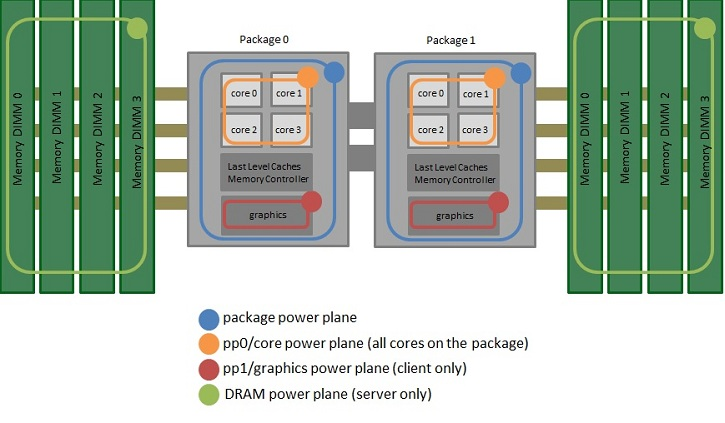
\includegraphics[width=1\textwidth]{images/power_domains2.jpg}


        \end{figure}

        \footnotesize{Source: https://software.intel.com/en-us/articles/intel-power-governor}


    \end{frame}


    %% %%%%%%%%%% %%%%%%%%%% %%%%%%%%%% %%%%%%%%%% %%%%%%%%%% %%%%%%%%%% %%%%%%%%%%

    \begin{frame}[fragile]{Benchmark execution and analysis}{Criterion}

        \begin{verbatim}
import Criterion.Main

-- Our benchmark harness.
main = defaultMain [
    bgroup "Map/" [
        env (...) -> bench addAllOpDesc $
            nf ( addAllNTimes a b ) addAllNRepeats
    ]
]
        \end{verbatim}


    \end{frame}


    %% %%%%%%%%%% %%%%%%%%%% %%%%%%%%%% %%%%%%%%%% %%%%%%%%%% %%%%%%%%%% %%%%%%%%%%

    \begin{frame}[fragile]{Benchmark execution and analysis}{Criterion}

        \begin{verbatim}
benchmarking (...)/addAll_1000_times_1000_elements_to_100000
time                 1.245 s    (1.234 s .. 1.261 s)
                     1.000 R^2   (1.000 R^2 .. 1.000 R^2)
mean                 1.248 s    (1.246 s .. 1.251 s)
std dev              3.883 ms   (0.0 s .. 4.130 ms)
packageEnergy:       1.000 R^2   (0.998 R^2 .. 1.000 R^2)
  iters              31.288     (29.594 .. 33.275)
  y                  0.545      (-2.154 .. 5.209)
dramEnergy:          1.000 R^2   (1.000 R^2 .. 1.000 R^2)
  iters              10.404     (10.214 .. 10.680)
  y                  0.121      (-0.262 .. 0.671)
        \end{verbatim}


    \end{frame}


    %% %%%%%%%%%% %%%%%%%%%% %%%%%%%%%% %%%%%%%%%% %%%%%%%%%% %%%%%%%%%% %%%%%%%%%%


%% %%%%%%%%%% %%%%%%%%%% %%%%%%%%%% %%%%%%%%%% %%%%%%%%%% %%%%%%%%%% %%%%%%%%%%


